\documentclass{ctexart}
\usepackage{graphicx}
\usepackage{caption}
\usepackage{float}
\usepackage{amsmath}
\usepackage{fancyhdr}
\usepackage{xunicode-addon}
\usepackage{booktabs}
\usepackage{listings}
\usepackage{hyperref}
\usepackage[a4paper,hmargin=1.25in,vmargin=1in]{geometry}
% !TeX program = xelatex
\lstdefinestyle{mystyle}{
  basicstyle=\ttfamily\footnotesize,
  breakatwhitespace=false,         
  breaklines=true,                 
  captionpos=b,                    
  keepspaces=true,                 
  numbers=left,                    
  numbersep=5pt,                  
  showspaces=false,                
  showstringspaces=false,
  showtabs=false,                  
  tabsize=2
}

\lstset{style=mystyle}

\title{\begin{figure}[H]
	\centering 
	\includegraphics[height=7cm,width=14cm]{E:/Pictures/中科大.jpg}
	\end{figure}\Huge\textbf{数据结构实验报告5}\\\huge{哈希表}}
\date{}
\punctstyle{banjiao} 
\pagestyle{fancy}
	\fancyhead[C]{\LARGE\textbf{实验报告5}}
	\fancyhead[L]{}
	\fancyhead[R]{}
	\fancyfoot[C]{\thepage}
\begin{document}
	\maketitle
	\thispagestyle{empty}
	
	\[\makebox{\Large{姓名:\underline{\makebox[5cm]{高茂航}}}}\]
	
    \[\makebox{\Large{学号:\underline{\makebox[5cm]{PB22061161}}}}\]
	
	\[\makebox{\Large{日期:\underline{\makebox[5cm]{2023年12月10日}}}}\]
	
	\clearpage

	\pagenumbering{arabic}

	\section{问题描述}
	1. 输入关键字序列;

	2. 用除留余数法构建哈希函数,用线性探测法(线性探测再散列)解决冲突,
	构建哈希表 HT1;

	3. 用除留余数法构建哈希函数,用拉链法(链地址法)解决冲突,构建哈希
	表 HT2;

	4. 分别对 HT1 和 HT2 计算在等概率情况下查找失败时的平均查找次数;

	5. 分别在 HT1 和 HT2 中查找给定的关键字,给出查找次数。
	
	\section{算法描述}
	\subsection{数据结构}
	\subsubsection{线性探测再散列法}
	\begin{lstlisting}[language=C++, caption=线性探测再散列法]
		typedef struct{
			int Address[MAXNUM];//哈希表地址
			int Keyword[MAXNUM];//哈希表关键字
			int keynum;//关键字个数
			int SuccessFind[MAXNUM]={0};//成功查找次数
			int FailFind[MAXNUM]={0};//失败查找次数
			float AveSuccess=0;//查找成功的平均查找次数
			float AveFail=0;//查找失败时在各个位置上的平均查找次数
		}HashTable;
	\end{lstlisting}

	\subsubsection{链地址法}
	\begin{lstlisting}[language=C++, caption=链地址法]
		typedef struct Node{
			int data;
			Node* next=NULL;
		}Node;
		typedef struct SuccessNode{
			int SuccessNum;
			SuccessNode* next=NULL;
		}SuccessNode;
		typedef struct{
			int Address[MAXNUM];//哈希表地址
			int keynum=0;//关键字个数
			Node* Link[MAXNUM];//哈希表链地址
			SuccessNode* SuccessLink[MAXNUM];//成功查找次数
			int FailFind[MAXNUM]={0};//失败查找次数
			float AveSuccess=0;//查找成功的平均查找次数
			float AveFail=0;//查找失败时在各个位置上的平均查找次数
		}HashTable;
	\end{lstlisting}

	\subsection{程序结构}
	\subsubsection{线性探测再散列法}
	\begin{lstlisting}[language=C++, caption=线性探测再散列法]
		int Hash(int);//哈希函数(除留余数法)
		void InsertHash1(HashTable*,int);//线性探测再散列把关键字插入哈希表
		void SearchHash1(HashTable*,int);//在哈希表中查找关键字
		void JudgeFail1(HashTable*);//求在每个地址查找失败时的最小散列次数
		int main(){
			int i,key[MAXNUM];
			HashTable *hashtable = new HashTable;
			cin>>hashtable->keynum;
			for(i=0;i<hashtable->keynum;i++)
				cin>>key[i];
			cin>>p;
			for(i=0;i<p;i++){
				hashtable->Address[i]=i;
				hashtable->Keyword[i]=-1;//初始化哈希表中没有关键字的位置为-1
			}
			cout<<"哈希表地址:";
			for(i=0;i<p;i++)
				cout<<hashtable->Address[i]<<"  ";
			for(i=0;i<hashtable->keynum;i++)
				InsertHash1(hashtable,key[i]);
			cout<<"表中关键字:";
			for(i=0;i<p;i++)
				if(hashtable->Keyword[i]!=-1)
					cout<<i<<":"<<hashtable->Keyword[i]<<" ";
			for(i=0;i<hashtable->keynum;i++)
				SearchHash1(hashtable,key[i]);
			cout<<"成功查找次数:";
			for(i=0;i<p;i++){
				cout<<i<<":"<<hashtable->SuccessFind[i]<<" ";
				hashtable->AveSuccess+=hashtable->SuccessFind[i];
			}
			JudgeFail1(hashtable);//求在每个地址查找失败时的最小散列次数
			cout<<"失败查找次数:";
			for(i=0;i<p;i++){
				cout<<i<<":"<<hashtable->FailFind[i]<<" ";
				hashtable->AveFail+=hashtable->FailFind[i];
			}
			cout<<"查找成功的平均查找次数:"<<hashtable->AveSuccess/hashtable->keynum<<endl<<"查找失败的平均查找次数:"<<hashtable->AveFail/p<<endl;
			delete hashtable;
		}
	\end{lstlisting}

	\begin{lstlisting}[language=C++, caption=把关键字插入哈希表]
InsertHash1(HashTable* H,int key){//用线性探测再散列把关键字插入哈希表
    int address=Hash(key);
    while (H->Keyword[address]!=-1)
        address=(address+1)%p;//线性探测再散列
    H->Keyword[address]=key;
}
	\end{lstlisting}
	\begin{lstlisting}[language=C++, caption=在哈希表中查找关键字]
void SearchHash1(HashTable* H,int key){//在哈希表中查找关键字
	int address=Hash(key),num=0;
	while (H->Keyword[address]!=key){
		num++;
		address=(address+1)%p;
		if(H->Keyword[address]==-1||address==Hash(key)){//假如查找到一个没有关键字的位置或者查找了一圈回到原来的位置,说明哈希表中没有该关键字
			cout<<"哈希表中没有该关键字"<<endl;
			break;
		}
	}
	H->SuccessFind[address]=++num;
}
	\end{lstlisting}
	\begin{lstlisting}[language=C++, caption=求在每个地址查找失败时的最小散列次数]
void JudgeFail1(HashTable* H){//求在每个地址查找失败时的最小散列次数
    int i,temp;
    for(i=0;i<p;i++){
        H->FailFind[i]++;
        temp=i;
        while (H->Keyword[temp]!=-1){
            temp=(temp+1)%p;
            if(H->Keyword[temp]!=H->Keyword[i])
                H->FailFind[i]++;
            else{
                H->FailFind[i]++;
                break;
            }
        }
    }
}
	\end{lstlisting}
	\subsubsection{链地址法}
	\begin{lstlisting}[language=C++, caption=链地址法]
		int main(){
			//前面与上述代码相同
			for(i=0;i<p;i++){
				hashtable->Address[i]=i;
				hashtable->Link[i]=NULL;
				hashtable->SuccessLink[i]=NULL;
			}
			for(i=0;i<hashtable->keynum;i++)
				InsertHash2(hashtable,key[i]);
			Node* pt[p];
			for(i=0;i<p;i++)
				pt[i]=hashtable->Link[i];
			cout<<"表中关键字:";
			for(j=0;j<p;j++){
				if(pt[j]){
					cout<<j<<"(";
					while(pt[j]){
						if(pt[j]->next){
							cout<<pt[j]->data<<" ";
							pt[j]=pt[j]->next;
						}
						else{
							cout<<pt[j]->data;
							break;
						}
					}
					cout<<") ";
				}
			}
			SuccessNode* pt2[p];
			for(i=0;i<hashtable->keynum;i++)
				SearchHash2(hashtable,key[i]);
			for(i=0;i<p;i++)
				pt2[i]=hashtable->SuccessLink[i];
			cout<<"成功查找次数:";
			for(j=0;j<p;j++){
				if(pt2[j]){
					cout<<j<<"(";
					while(pt2[j]){
						if(pt2[j]->next){
							cout<<pt2[j]->SuccessNum<<" ";
							pt2[j]=pt2[j]->next;
						}
						else{
							cout<<pt2[j]->SuccessNum;
							break;
						}
					}
					cout<<") ";
				}
				else
					cout<<j<<"(0) ";
			}
			//后面与上述代码相同
		}
	\end{lstlisting}
	\begin{lstlisting}[language=C++, caption=把关键字插入哈希表]
	void InsertHash2(HashTable* H,int key){//链地址法把关键字插入哈希表
		int address=Hash(key);
		Node* newNode = new Node;
		newNode->data = key;
		newNode->next = NULL;
		if(!H->Link[address])
			H->Link[address] = newNode;
		else {
			Node* pt = H->Link[address];
			while (pt->next) 
				pt = pt->next;
			pt->next = newNode;
		}
	}
	\end{lstlisting}

	\begin{lstlisting}[language=C++, caption=在哈希表中查找关键字]
void SearchHash2(HashTable* H,int key){//在哈希表中查找关键字
    int address=Hash(key),num=0;
    Node* pt=H->Link[address];
    if(!pt){
        cout<<"哈希表中没有该关键字"<<endl;
        return;
    }
    while(pt){
        num++;
        if(pt->data == key){
            if(!H->SuccessLink[address]){
                SuccessNode* newNode = new SuccessNode;
                newNode->SuccessNum=num;
                newNode->next = NULL;
                H->AveSuccess+=num;
                H->SuccessLink[address]=newNode;
            }
            else {
                SuccessNode* pt2 = H->SuccessLink[address];
                SuccessNode* newNode = new SuccessNode;
                newNode->SuccessNum=num;
                newNode->next = NULL;
                H->AveSuccess+=num;
                while (pt2->next) 
                    pt2 = pt2->next;
                pt2->next = newNode;
            }
            return;
        }
        pt = pt->next;
    }
    cout<<"哈希表中没有该关键字"<<endl;   
}
	\end{lstlisting}
	\begin{lstlisting}[language=C++, caption=求在每个地址查找失败时的最小散列次数]
void JudgeFail2(HashTable* H){//求在每个地址查找失败时的最小散列次数
    int i,temp;
    for(i=0;i<p;i++){
        H->FailFind[i]++;
        if(H->Link[i]){
            Node* pt=H->Link[i];
            while(pt){
                H->FailFind[i]++;
                pt=pt->next;
            }
        }
    }
}
	\end{lstlisting}

	\subsubsection{哈希函数}
	\begin{lstlisting}[language=C++, caption=哈希函数(除留余数法)]
		int p=1;//除留余数法中的除数
		int Hash(int m){//哈希函数(除留余数法)
			return m%p;
		}
	\end{lstlisting}
	
	\section{调试分析}
	本程序遇到的主要问题是:

	1.在线性探测再散列查找失败时判断哈希表中是否存在该关键字的方法;

	2.在链地址法中,处理指针时出现Segmentation fault错误。

	但在插入关键字时,由于已经默认了插入的关键字互不相同,没有判断哈希表中是否已经存在该关键字。
	\section{算法时空分析}
	哈希表的空间复杂度是$O(n)$,插入查找的时间复杂度是$O(n)$,线性探测再散列的平均查找成功和失败次数一般大于链地址法。
	\section{测试结果分析}
	\subsection{线性探测探测再散列法}
	\begin{figure}[H]
	\centering 
	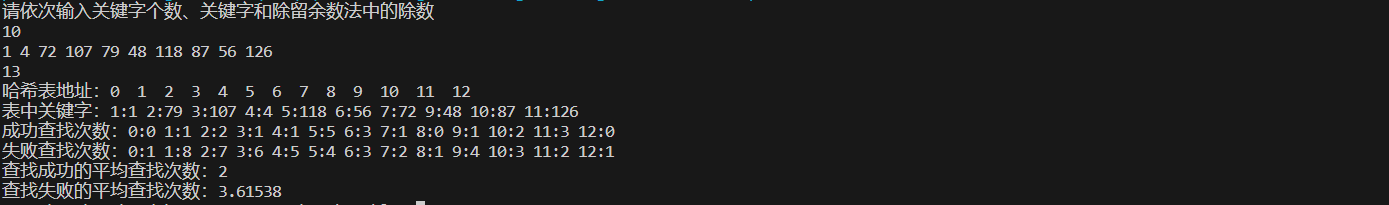
\includegraphics[height=2.5cm,width=14cm]{1.png}
	\end{figure}
	\begin{figure}[H]
	\centering 
	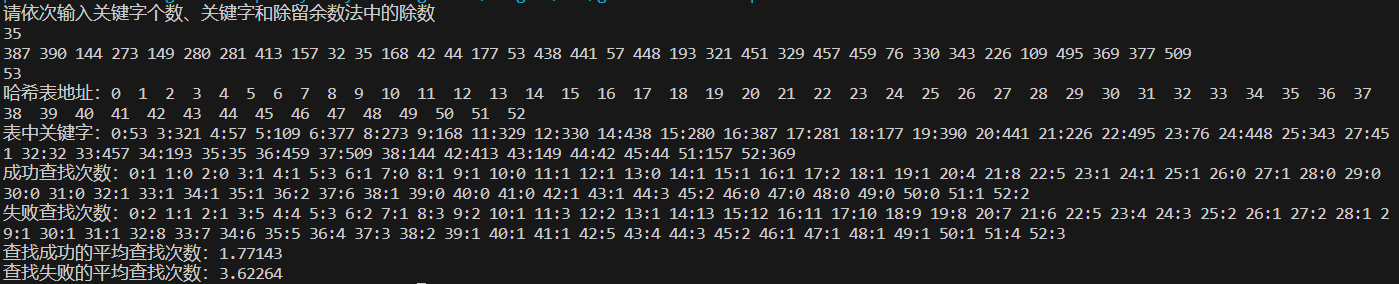
\includegraphics[height=3cm,width=14cm]{2.png}
	\end{figure}
	\begin{figure}[H]
	\centering 
	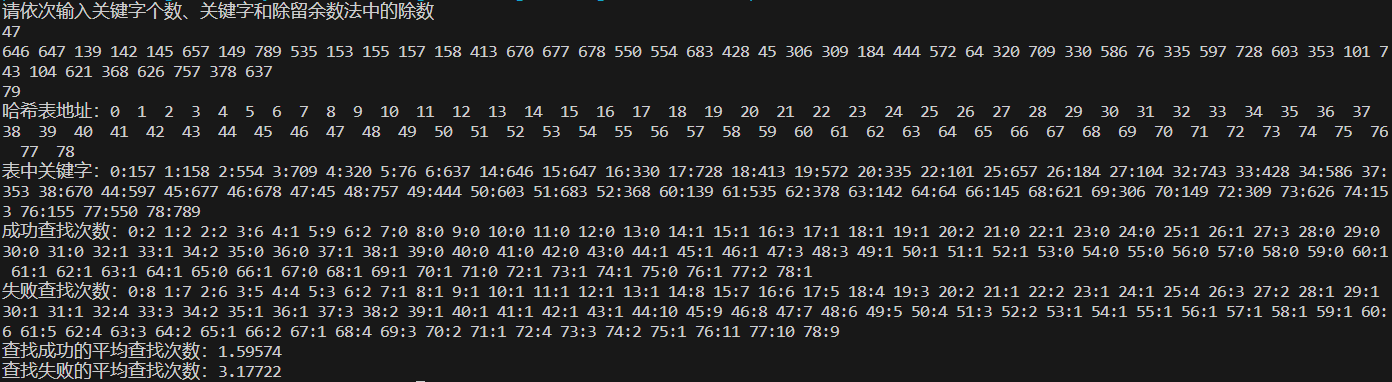
\includegraphics[height=3.5cm,width=14cm]{3.png}
	\end{figure}
	
	\subsection{链地址法}
	\begin{figure}[H]
	\centering 
	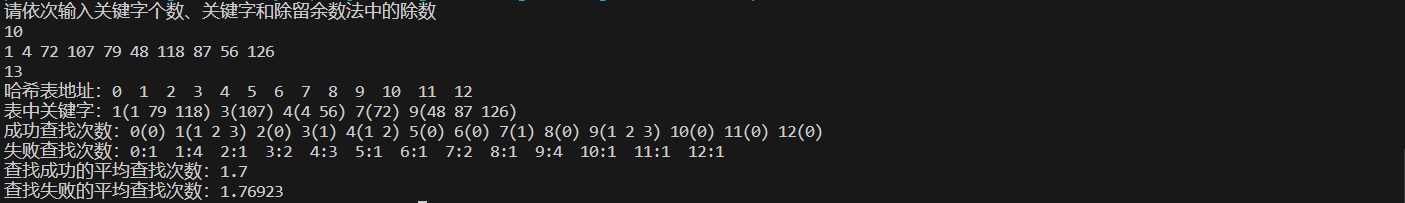
\includegraphics[height=2cm,width=14cm]{7.png}
	\end{figure}
	\begin{figure}[H]
	\centering 
	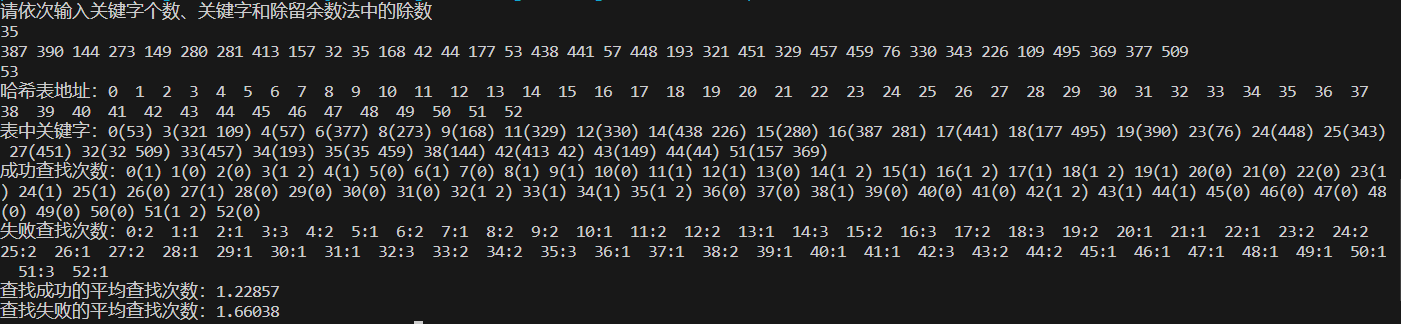
\includegraphics[height=3.5cm,width=14cm]{8.png}
	\end{figure}
	\begin{figure}[H]
	\centering 
	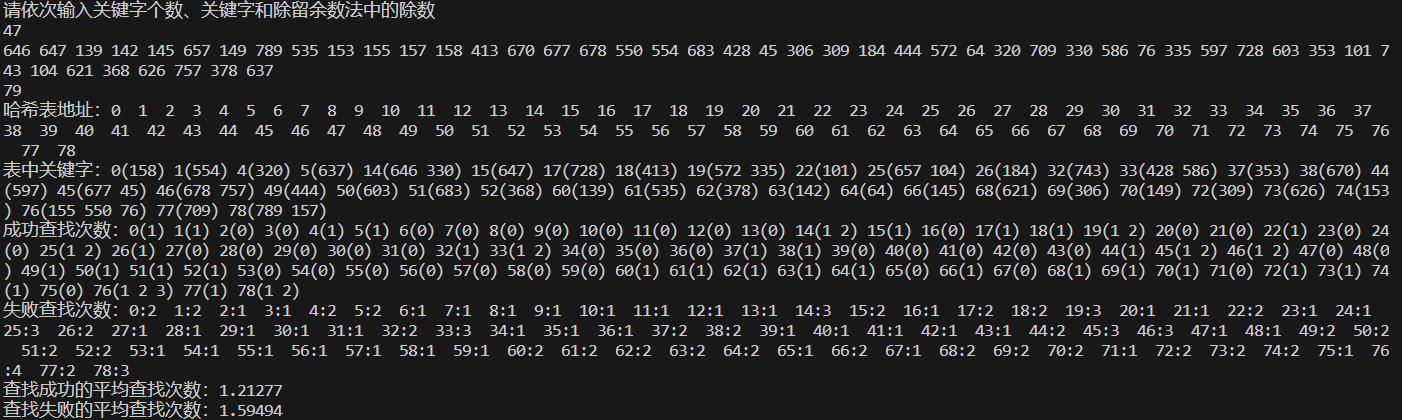
\includegraphics[height=4.5cm,width=14cm]{9.png}
	\end{figure}
\section{实验体会收获}
   通过本次实验掌握了用除留余数法构建哈希表、用线性探测再散列法和链地址法处理冲突的方法,
   加深了对哈希表和查找相关知识的认识。

\end{document}